\documentclass[letterpaper,11pt]{article}

\usepackage[spanish]{babel}
\usepackage[top=2cm,bottom=2cm,right=2cm,left=2cm]{geometry}
\usepackage{amssymb}
\usepackage{amsmath}
\usepackage{amsthm}
\usepackage{empheq}
\usepackage{mdframed}
\usepackage{booktabs}
\usepackage{lipsum}
\usepackage{graphicx}
\usepackage{color}
\usepackage{psfrag}
\usepackage{pgfplots}
\usepackage{bm}
\usepackage{multicol}
\usepackage{wrapfig}
\usepackage{float}
\usepackage{wrapfig}
\usepackage{multirow}
\usepackage{biblatex}
\usepackage{csquotes}
\usepackage{parskip}
\usepackage{cancel}
\usepackage{listing}
\usepackage{tikz}
\usepackage{verbatim}
\usepackage{subcaption}
\usepackage{enumitem}
\usepackage{xcolor}
\usepackage{xfrac}

\graphicspath{{fig/}}
\addbibresource{biblio.bib}
\usepgfplotslibrary{colorbrewer}
\pgfplotsset{width=8cm,compat=1.9}
\definecolor{negro}{RGB}{0,0,0}
\definecolor{azul}{RGB}{0,0,255}
\definecolor{verde}{RGB}{0,255,0}
\definecolor{cian}{RGB}{0,255,255}
\definecolor{rojo}{RGB}{255,0,0}
\definecolor{magenta}{RGB}{255,0,255}
\definecolor{amarillo}{RGB}{255,255,0}
\definecolor{blanco}{RGB}{255,255,255}

\definecolor{limegreen}{cmyk}{0.75,0,1,0}
\definecolor{orange}{cmyk}{0,0.8,0.95,0}
\definecolor{purple}{cmyk}{0.75,1,0,0}

\begin{document}

\onecolumn\begin{@twocolumntrue}
    \begin{minipage}{0.3\textwidth}{
\includegraphics[scale=0.24]{Escudo_UD.pdf}} % Cambiar escudo
    \end{minipage}
    \vspace{10pt}
    \begin{minipage}{0.677\textwidth}
        \begin{center}
            \vspace{12mm}
        
            \Large{\textbf{Tarea 3: osciladores y ecuaciones diferenciales}}
            \vspace{3mm}
            
            \large{\textbf{Juan Sebastian Manrique Moreno}}
            \vspace{2mm}
    
            \large{\textit{Ecuaciones diferenciales, Programa Académico de Física, Universidad Distrital Francisco José de Caldas}}
            \vspace{1mm}
            
            Octubre de 2022 % Formato (mes) de (año)
        \end{center}
\vspace{5pt}
\end{minipage}

\centerline{\rule{0.95\textwidth}{0.4pt}} % Línea negra
\end{@twocolumntrue}

\begin{multicols}{2}

\section*{Ejercicio:}

Suponga el siguiente sistema masa-resorte con 3 masas acopladas:

\begin{figure}[H]
\begin{center}
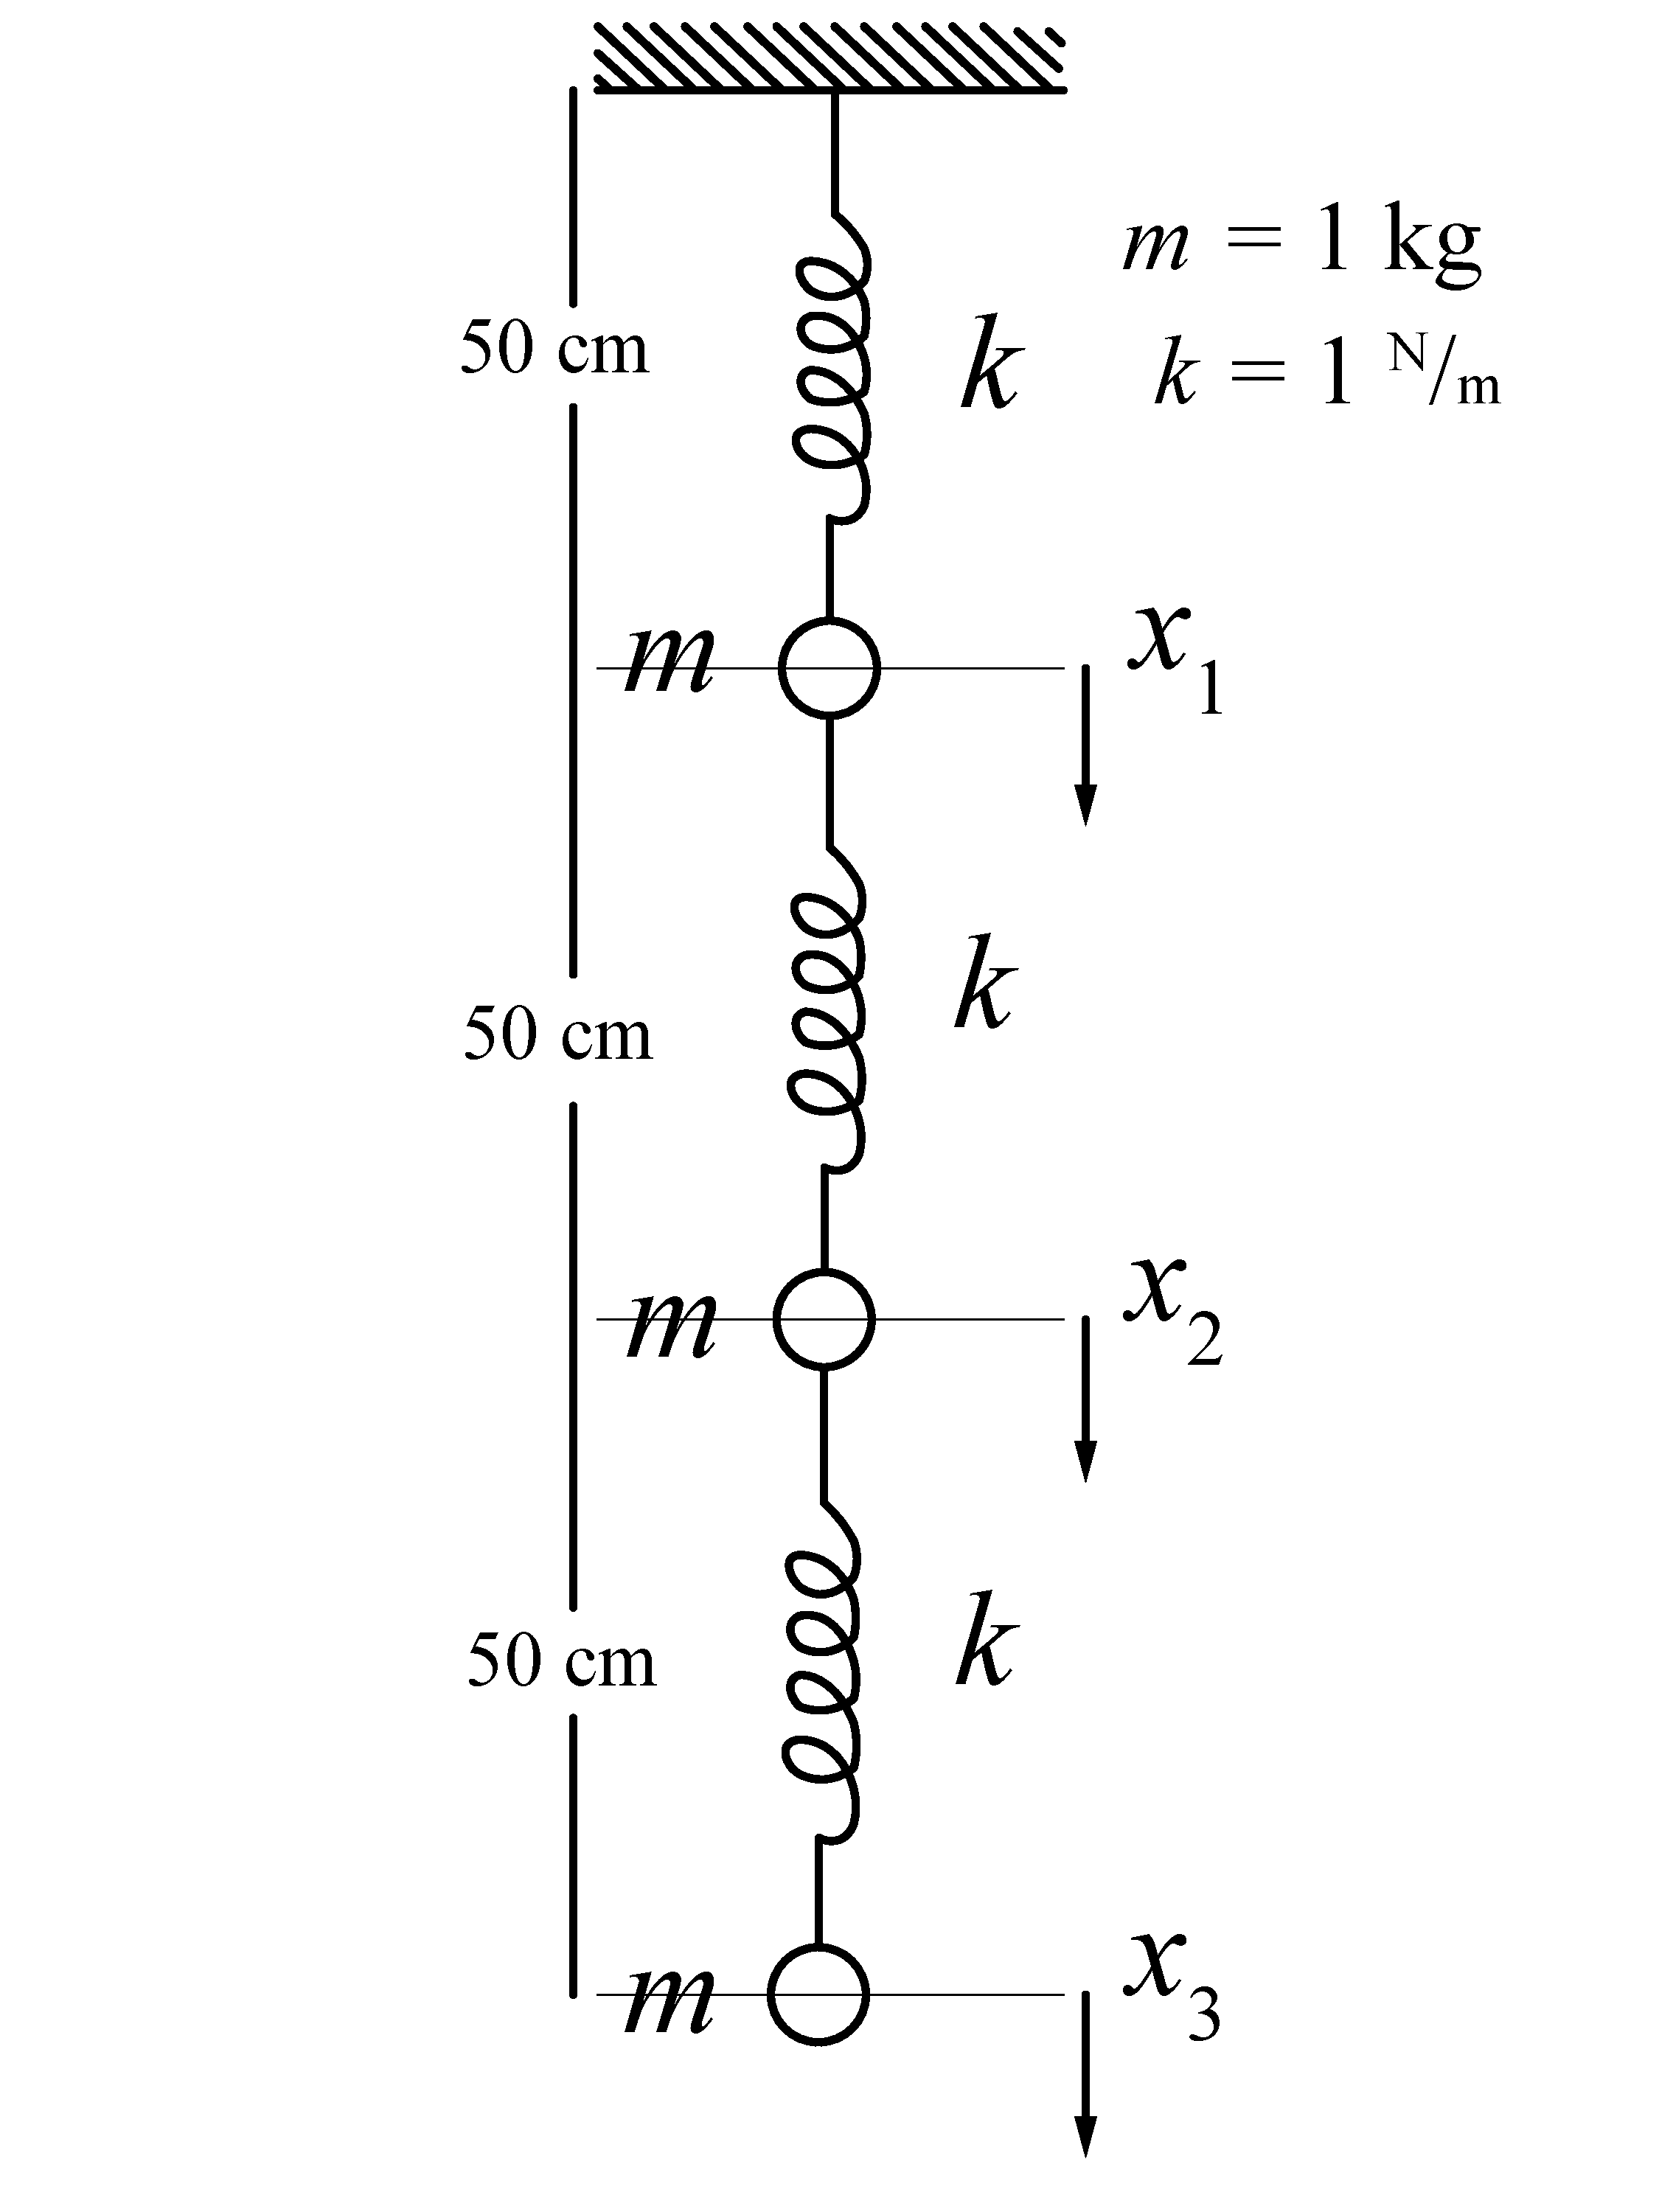
\includegraphics[scale=0.2]{sistema.pdf}
\caption{Sistema masa-resorte con 3 masas acopladas}
\label{fig:1}
\end{center}
\end{figure}

Teniendo en cuenta la Figura \ref{fig:1}:

\begin{enumerate}[leftmargin=15pt]
    \item Realizar el diagrama de cuerpo libre.
    \item Plantear el sistema de ecuaciones diferenciales del sistema.
    \item Organizar las ecuaciones y realizar las definiciones pertinentes.
    \item Suponer soluciones especiales para el sistema de ecuaciones y reemplazarlas en el mismo.
    \item Escribir la ecuación matricial para las frecuencias y amplitudes.
    \item Encontrar las frecuencias de los modos normales del sistema (determinante de $W = 0$).
    \item Encontrar las relaciones de amplitud para el sistema.
\end{enumerate}

\subsubsection*{Solución:}

\begin{enumerate}[leftmargin=15pt]
    \item El diagrama de cuerpo libre es:
    \begin{figure}[H]
        \begin{center}
        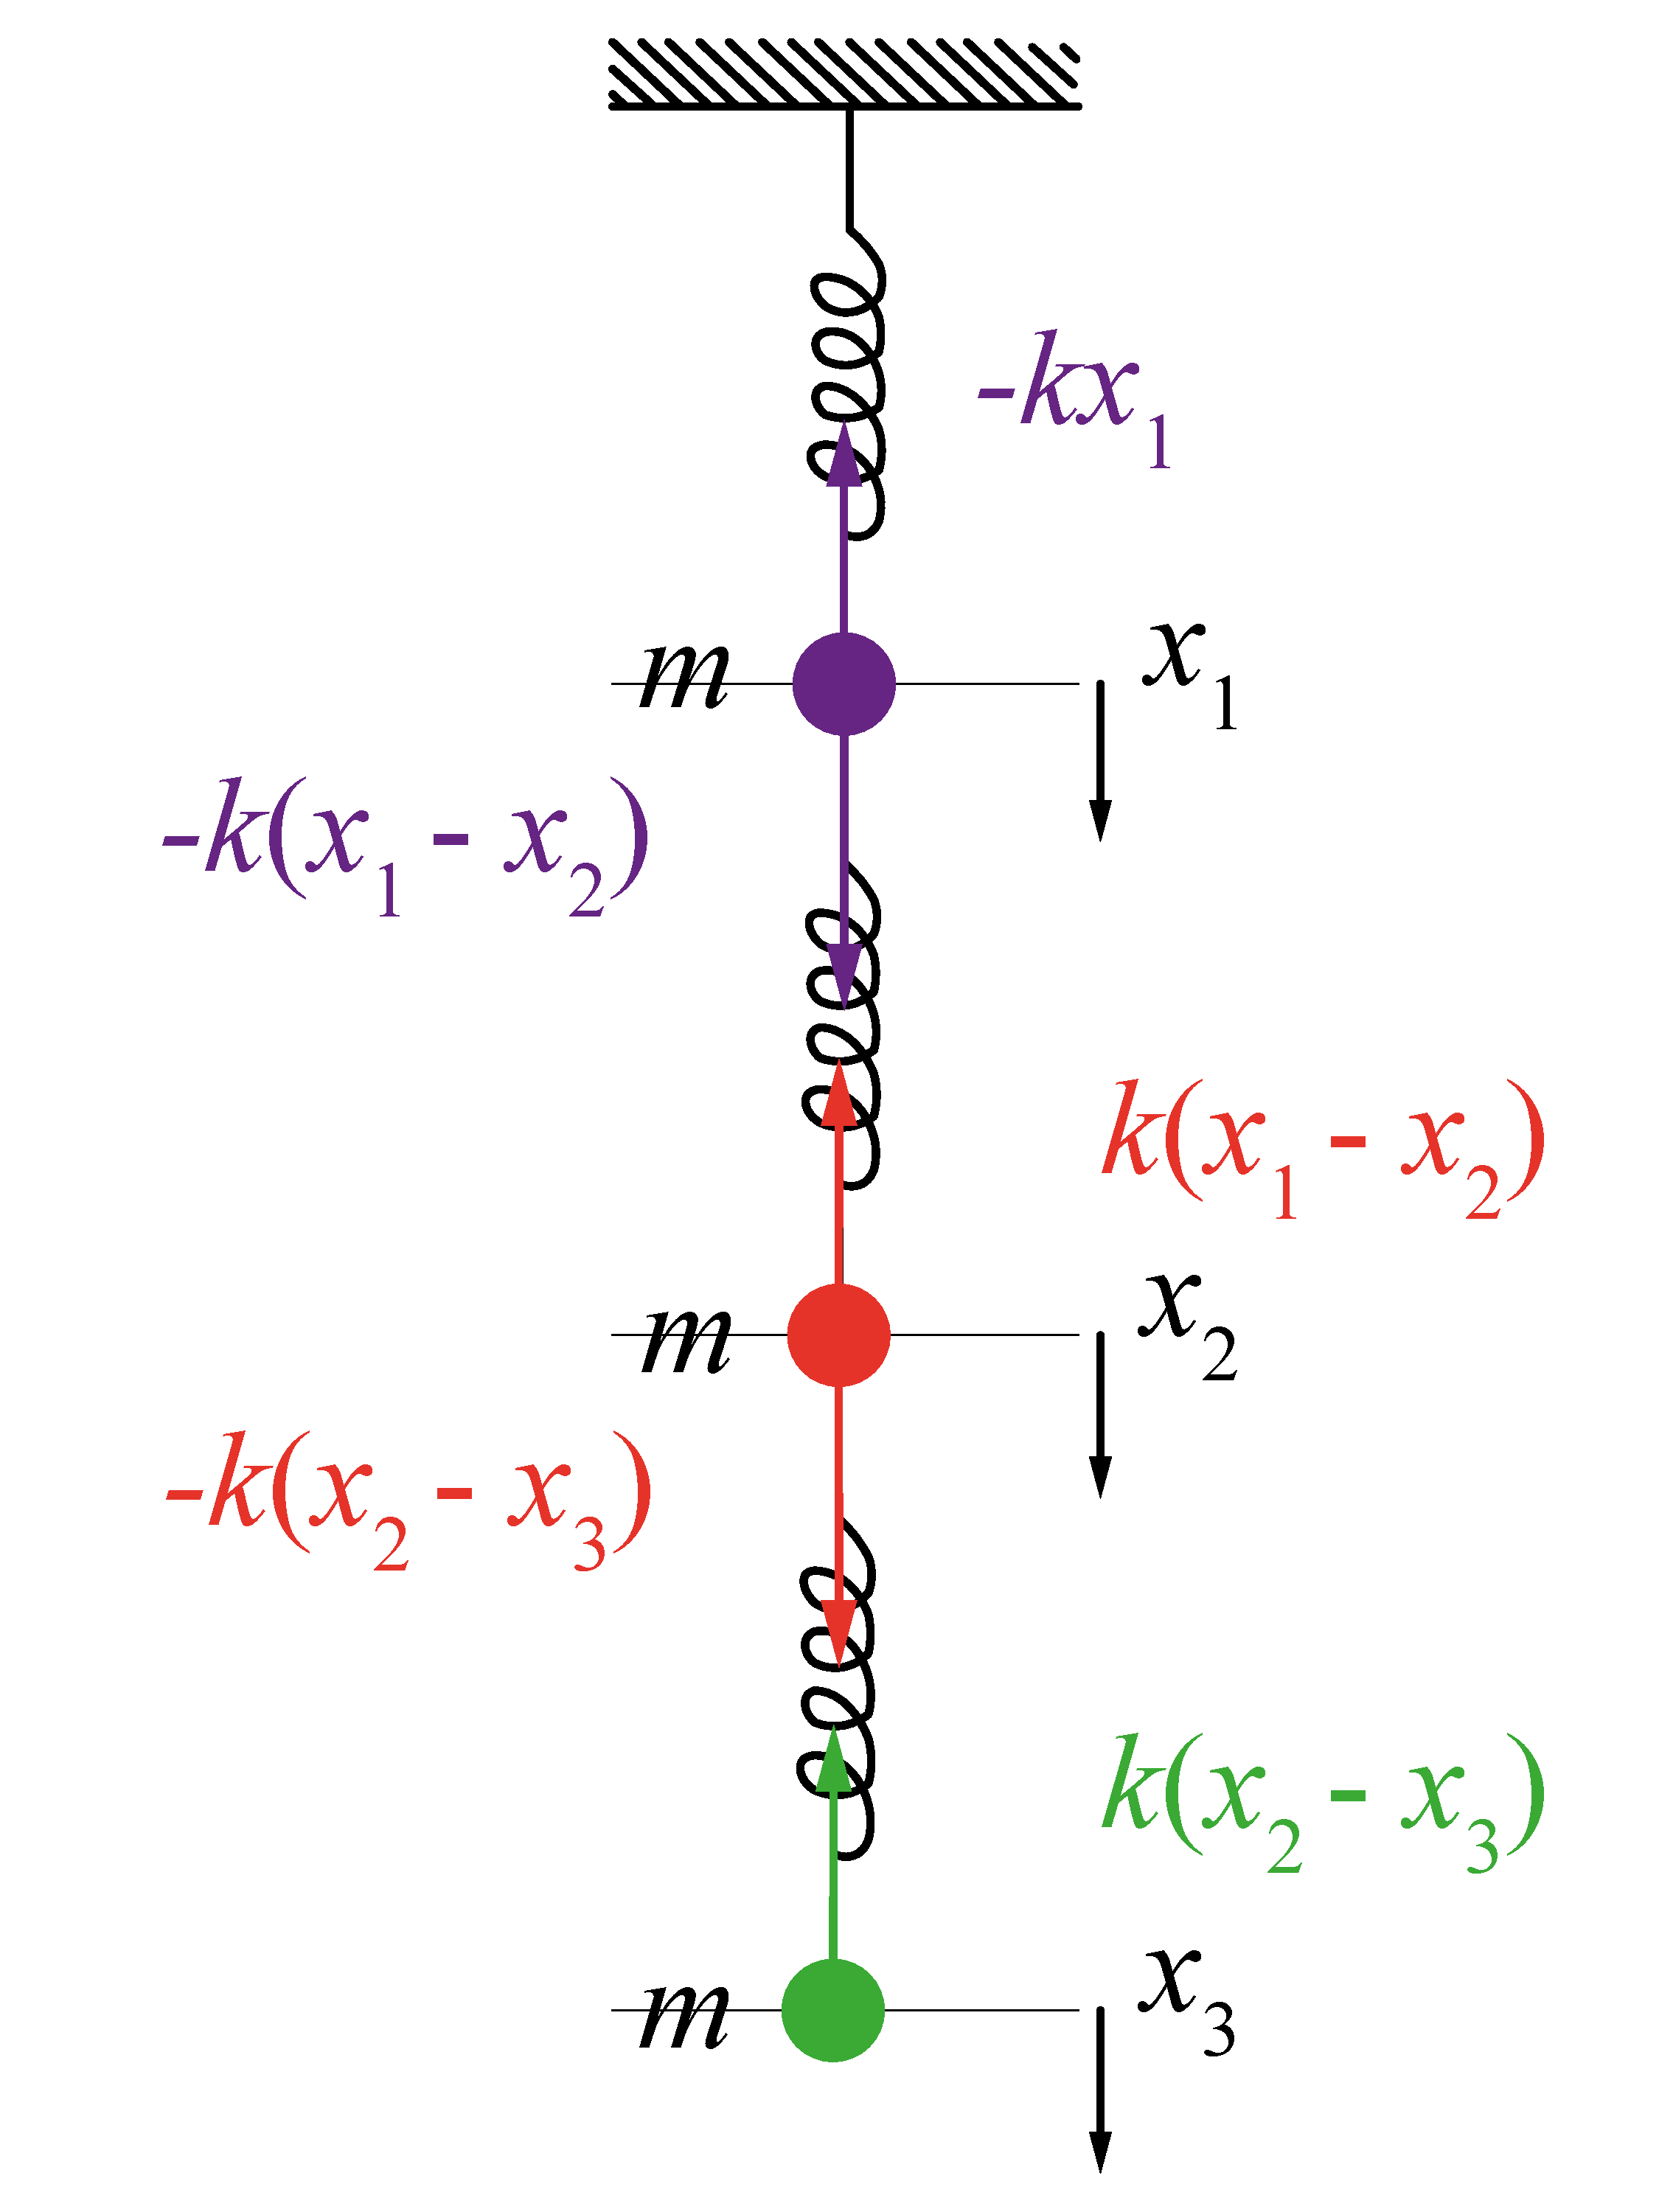
\includegraphics[scale=0.18]{diagrama.pdf}
        \caption{<<Comentario figura>>}
        \label{diagrama}
        \end{center}
    \end{figure}
    \item Teniendo en cuenta la Figura \ref{diagrama}, el sistema de ecuaciones diferenciales es:
    \begin{equation*}
        \begin{cases}
            &m \displaystyle\frac{d^{2}x_{1}}{dt^{2}} = -kx_{1} - k(x_1 - x_2)\\
            \\
            &m \displaystyle\frac{d^{2}x_{2}}{dt^{2}} = k(x_1 - x_2) - k(x_2 - x_3)\\
            \\
            &m \displaystyle\frac{d^{2}x_{3}}{dt^{2}} = k(x_2 - x_3)
        \end{cases}
    \end{equation*}
    \item La cual se reescribe teniendo las ecuaciones diferenciales de la forma general, por tanto:
    \begin{equation*}
        \begin{cases}
            &m \displaystyle\frac{d^{2}x_{1}}{dt^{2}} + kx_{1} + k(x_1 - x_2) = 0\\
            \\
            &m \displaystyle\frac{d^{2}x_{2}}{dt^{2}} - k(x_1 - x_2) + k(x_2 - x_3) = 0\\
            \\
            &m \displaystyle\frac{d^{2}x_{3}}{dt^{2}} - k(x_2 - x_3) = 0
        \end{cases}
    \end{equation*}
    Ya que,
    \begin{align*}
        \omega^{2}_{0} = \frac{k}{m}
    \end{align*}
    donde $m$ es la masa y $k$ la constante de elasticidad del resorte, podemos dividir las 3 ecuaciones diferenciales por $m$, de esta manera nos queda un sistema con ecuaciones diferenciales con soluciones conocidas y además en función de las frecuencias, sin embargo, conocemos valores para $k$ y $m$ por lo que conocemos el valor para $\omega^{2}_{0}$, entonces:
    \begin{align*}
        \omega^{2}_{0} = \frac{1~\sfrac{\mathrm{N}}{\mathrm{m}}}{1~\mathrm{kg}} \Rightarrow \omega^{2}_{0} = 1~\mathrm{s}^{-2}
    \end{align*}
    De esta manera, el sistema de ecuaciones diferenciales resulta:
    \begin{equation*}
        \begin{cases}
            &\textcolor{rojo}{\displaystyle\frac{d^{2}x_{1}}{dt^{2}} + x_{1} \cdot \mathrm{s}^{-2} + (x_1 - x_2) \cdot \mathrm{s}^{-2} = 0}\\
            \\
            &\textcolor{rojo}{\displaystyle\frac{d^{2}x_{2}}{dt^{2}} - (x_1 - x_2) \cdot \mathrm{s}^{-2} + (x_2 - x_3) \cdot \mathrm{s}^{-2} = 0}\\
            \\
            &\textcolor{rojo}{\displaystyle\frac{d^{2}x_{3}}{dt^{2}} - (x_2 - x_3) \cdot \mathrm{s}^{-2} = 0}
        \end{cases}
    \end{equation*}
    Se colocan las unidades para demostrar que existen las frecuencias inclusive si estas valen 1.
    \item Debido a la forma de las ecuaciones diferenciales, ya conocemos sus soluciones generales, por tanto, esas mismas soluciones se van a suponer con tal suerte que satisfagan el sistema de ecuaciones.
    
    La solución general es:
    \begin{align}
        x^{n} = D_n \cos\left(\omega_n t + \delta_n\right) \label{eq:1}
    \end{align}
    De esta manera las soluciones especiales para las ecuaciones diferenciales son:
    \begin{equation*}
        \begin{cases}
            &\textcolor{rojo}{x^{n}_{1} = D_{1n} \cos\left(\omega_n t + \delta_n\right)}\\
            \\
            &\textcolor{rojo}{x^{n}_{2} = D_{2n} \cos\left(\omega_n t + \delta_n\right)}\\
            \\
            &\textcolor{rojo}{x^{n}_{3} = D_{3n} \cos\left(\omega_n t + \delta_n\right)}
        \end{cases}
    \end{equation*}
    Derivando dos veces (\ref{eq:1}) para comprobar si es solución, tomando $\mathscr{C} = \cos\left(\omega_n t + \delta_n\right)$:
    \begin{align*}
        x^{n}_{1} &= D_{1n} \mathscr{C}, & \ddot{x}^{n}_{1} &= -\omega^{2}_{n} D_{1n} \mathscr{C}\\
        x^{n}_{2} &= D_{2n} \mathscr{C}, & \ddot{x}^{n}_{2} &= -\omega^{2}_{n} D_{2n} \mathscr{C}\\
        x^{n}_{3} &= D_{3n} \mathscr{C}, & \ddot{x}^{n}_{3} &= -\omega^{2}_{n} D_{3n} \mathscr{C}
    \end{align*}
    Reemplazando los valores para $x$ en cada ecuación por separado donde ya conociendo las unidades para la frecuencia y sabiendo que está implícita no se colocará, resulta:

    Para $x^{n}_{1}$:
    \begin{align*}
        \cancel{\mathscr{C}}\left[-\omega^{2}_{n} D_{1n}  + D_{1n} + (D_{1n} - D_{2n})\right] &= 0\\
        D_{1n} \left(2 - \omega^{2}_{n}\right) - D_{2n} &= 0
    \end{align*}
    Para $x^{n}_{2}$:
    \begin{align*}
        \cancel{\mathscr{C}} \left[-\omega^{2}_{n} D_{2n} - \left(D_{1n} - D_{2n}\right) + \left(D_{2n} - D_{3n}\right)\right] &= 0\\
        - D_{1n} + D_{2n}\left(3 - \omega^{2}_{n}\right) - D_{3n} &= 0
    \end{align*}
    Para $x^{n}_{3}$:
    \begin{align*}
        \cancel{\mathscr{C}} \left[-\omega^{2}_{n} D_{3n} - \left(D_{2n} - D_{3n}\right)\right] &= 0\\
        - D_{2n} + D_{3n}\left(1 - \omega^{2}_{n}\right) &= 0
    \end{align*}
    Ya teniendo los valores reemplazados, se puede hallar la forma matricial de los resultados.
    \item La \textcolor{rojo}{forma matricial} para el sistema de ecuaciones diferenciales es:
    \begin{equation*}
        \begin{vmatrix}
        2 - \omega^{2}_{n} & -1 & 0\\
        -1 & 3 - \omega^{2}_{n} & -1\\
        0 & -1 & 1 - \omega^{2}_{n}
        \end{vmatrix}
        \cdot
        \begin{vmatrix}
            D_{1n} \\
            D_{2n} \\
            D_{3n} 
        \end{vmatrix}
        =
        \begin{vmatrix}
            0 \\
            0 \\
            0 
        \end{vmatrix}
    \end{equation*}
    Para que el sistema tenga solución, el determinante de la forma matricial mostrada debe ser igual a 0, por tanto:
    \begin{align*}
        \left(2 - \omega^{2}_{n}\right)\left[\left(3 - \omega^{2}_{n}\right)\left(1 - \omega^{2}_{n}\right) - 1\right] + \omega^{2}_{n} - 1 &= 0
    \end{align*}
\end{enumerate}


\end{multicols}

\end{document}